% A sample model to write a TFG project

% IMPORTANT!!! Substitute "draft" with "final" to render the final version of the TFG 
\documentclass[titlepage,openright,twoside,a4paper,final,12pt,spanish]{book}

% Configuring the environment to support spanish characters.
\usepackage[T1]{fontenc}
\usepackage[utf8]{inputenc}
\usepackage[english]{babel}
\selectlanguage{english}

\usepackage[pdftex,final]{graphicx}

% Style package
\usepackage{trinidad-TfG}
% Font Package (Palatino)
\usepackage{mathpazo}
% Packages for specific capabilities
\usepackage{rotating} % for text rotation in tables
\usepackage{multirow} % for multirow in tables
\usepackage{subfigure} % Place subfigures in figure environment
% Packages for specific symbols
\usepackage{amssymb}
\usepackage{amsmath}
\usepackage{amsfonts}
\usepackage{eurosym} % Euro symbol
\usepackage{bbding} % for \XSolidBrush
\usepackage{pifont} % for \ding{55} (a check mark)

\usepackage{float}
\author{Álvaro González Jiménez}{Grado en Ingeniería Informática - Ingeniería del Software}{D.~}{53585603L}
\authorURL{https://github.com/alvarogonjim}
\authorEMail{alvgonjim1@alum.us.es}
\setTitle{Deep learning for Image Classification}
%\setSubtitle{No subtitle}
\setUniversity{Universidad de Sevilla}

\supervisor{Isabel A. Nepomuceno Chamorro}{Dr.~}{Lenguajes y Sistemas Informáticos}



\makeglossaries
\begin{document}
\makeTitlePage

\pagestyle{empty}
\begin{dedication}
Tu dedicatoria aquí
\end{dedication}
\pagenumbering{roman}
\pagestyle{trinidadPhD}

\chapter*{Agradecimientos}

No olvides añadir una nota de agradecimiento a quienes hayan contribuido emocionalmente al proyecto fin de Grado.

\tableofcontents
\listoffigures
\listoftables
\listoftodos
\newpage

\pagenumbering{arabic}

\lineNumbersOn
\part{Introducción}
%!TEX root =  tfg.tex
\chapter{Motivation and problem definition}

\begin{abstract}
In this chapter, we will present the problem that we are going to solve in the futures chapters. Furthermore, we will explain my motivation in order to choose this topic. 
\end{abstract}

\section{Motivation and objectives}

During my last year of degree I was wondering what I was going to work on my thesis. I knew I wanted to work on something related to health because I had always been interested in creating a product with value which would have an impact on society.

During my internship I was in one of the most important research centres in France, \href{http://www.europe.naverlabs.com}{Naver Labs Europe}, in the field of artificial intelligence. There I realized the potential of the Deep Learning technology that was emerging during these years. I could do something related to health that I had not worked previously during my studies.

As a responsible software engineer I will build a maintainable software following the rules and standards that I learned during these years, as well as learn new emerging technologies. Although the result will not be as good as  
recent studies because of the available resources.

The main objective is to learn about this technology that I have never studied before and achieve a scalable prototype whose precision and quality will increase in the future using different techniques. We will compare the obtained results with other algorithms and/or other works (papers, studies and so on). Finally, we are going to expose the best model in a REST API so we can build an APP which sends a picture, taken from the camera, as an input to the API and it will return the predicted results to the user.


\section{Definition of the problem}
``Nowadays the melanoma of the skin represents 5.3\% of all new cancer cases in the U.S. In 2018, it is estimated that there will be 91,270 new cases of melanoma of the skin and an estimated 9,320 people will die of this disease'' \cite{melanoma-stadistics}. A quickly prediction of this disease will help to reduce the number of die people. In fact, most of the people do not realize that they have melanoma of the skin so it will make harder the cure process. 

\begin{figure}[H]
\centering
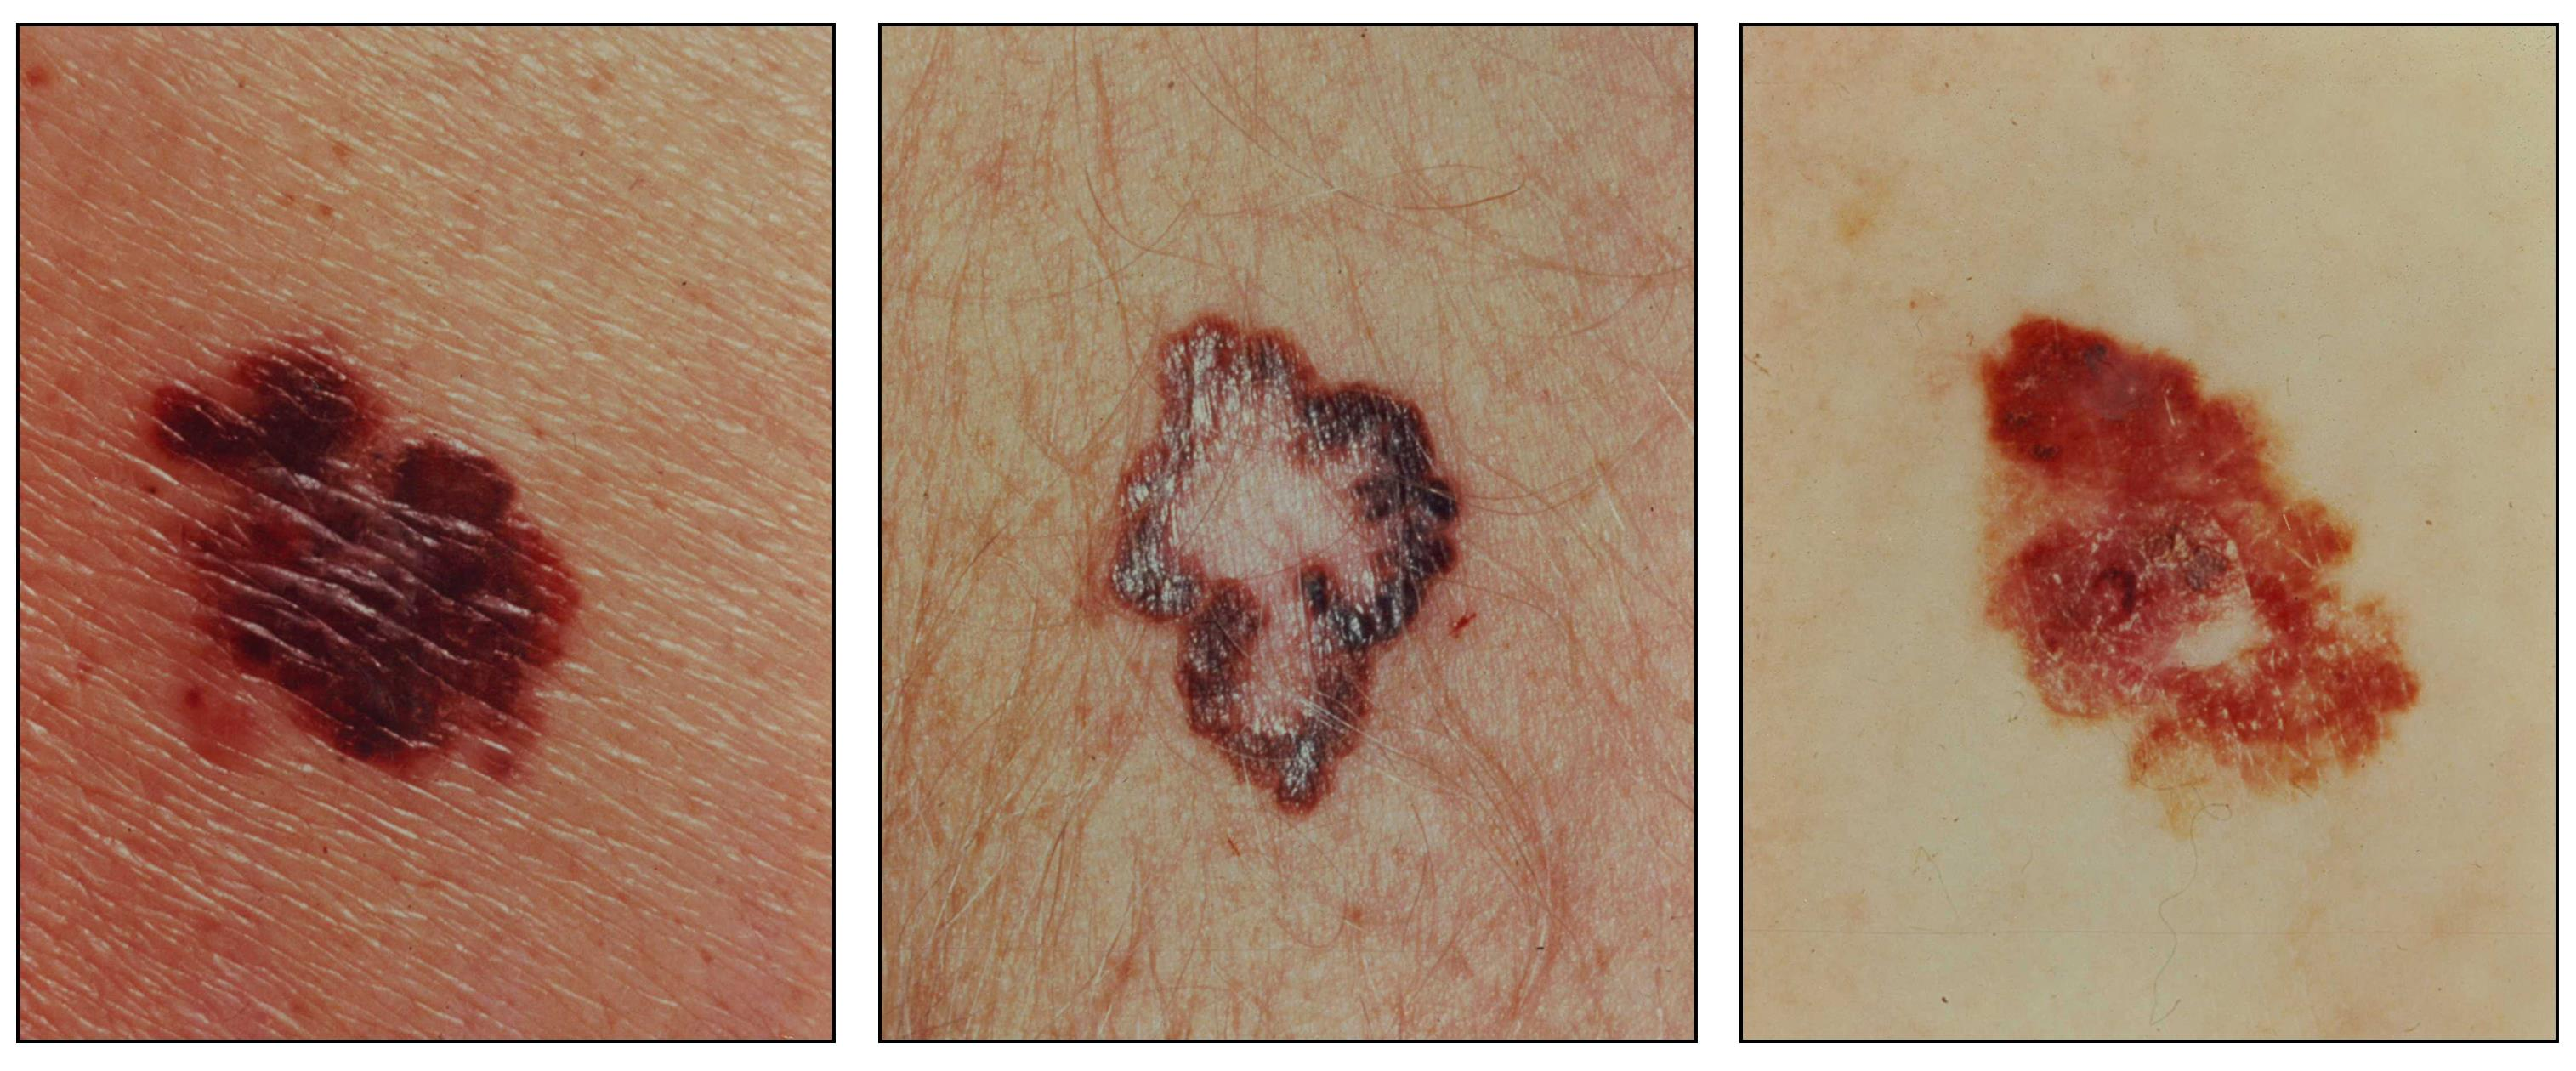
\includegraphics[width=0.8\textwidth]{./figures/melanoma-examples.jpg}
\caption{Examples of melanoma of the skin. \cite{melanoma-stadistics}}
\label{fig:jobInformationDialog}
\end{figure}

As you can see in the figure ~\ref{fig:jobInformationDialog} the melanoma presents a wide variety of characteristics, for example the pigmentation of the skin will be dark, the size is bigger than the normal pigmentation of the skin and the shape is irregular. This set of characteristics make a difficult task for human eye but an interesting research line using AI algorithms to detect the melanoma. 


\chapter{AI History and State of the art}

\begin{abstract}
In this chapter, we will explore a little bit about the Machine Learning world, 
the algorithms that people have been used for years to solve this and other types of problems. A brief summary about the current frameworks that we can use to solve this problem, theirs pros and cons. Finally we are going to explain the problems that we are going to solve. 
\end{abstract}


\section{Artificial Intelligence History}

Deep Learning (DL) has revolutionized industry after industry. People thinks that Deep Learning and Artificial Intelligence (AI) are synonyms, but these words are totally different.
We can define the AI as \emph{the automation of intellectual tasks normally performed by humans}.
The AI started in the beginning of the 1957 when John McCarthy held the first academic conference on the subject, the AI machines were able to solve problems that were difficult for humans to solve.

One of the most important AI machines in the history is the Enigma machine built by Alan Turin at the end of World War II. 
This machine could crack in hours entire conversations and text made by the Nazis.

In the early years of AI, a lot of researchers believed that AI could be achieved by hard coding rules. The kind of AI is called symbolic AI and was useful in solving well-defined, logical problems but it was incapable of solving complex problems such as image recognition, object detection, object segmentation, language translation, and natural-language-understanding.

In order to understand the relationship among AI, ML and DL let's visualize them as concentric circles see in the figure ~\ref{fig:iacircles}.


\begin{figure}[H]
\centering
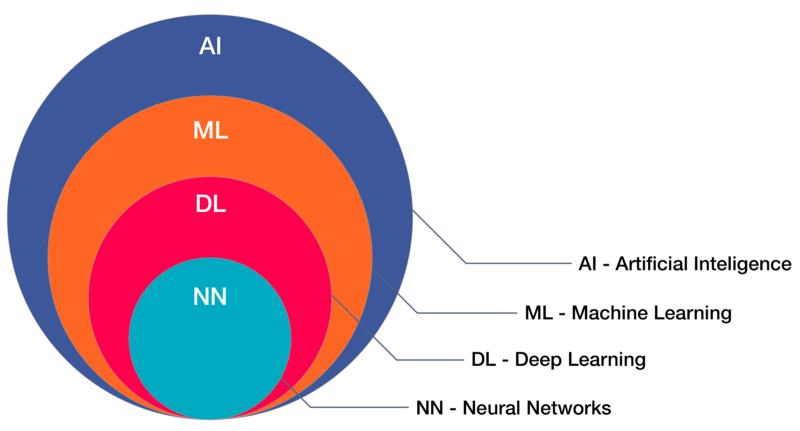
\includegraphics[width=0.8\textwidth]{./figures/ai-ml-dl}
\caption{Representation AI, ML and DL \cite{ai-ml-dl-image}}
\label{fig:iacircles}
\end{figure}

The idea that came first (AI) and the largest one. Then machine learning (ML) which blossomed later, and finally DL which is driving today's AI explosion (fitting inside both).

\subsection[Machine Learning]{Machine Learning}
Machine Learning (ML) is a sub-field of AI and has become very popular in the last 10 years. This discipline uses mathematics and statistics with the power of the computer to build intelligent systems that can learn by themselves, identify patterns and they are able to make decision without human intervention.

\begin{figure}[H]
\centering
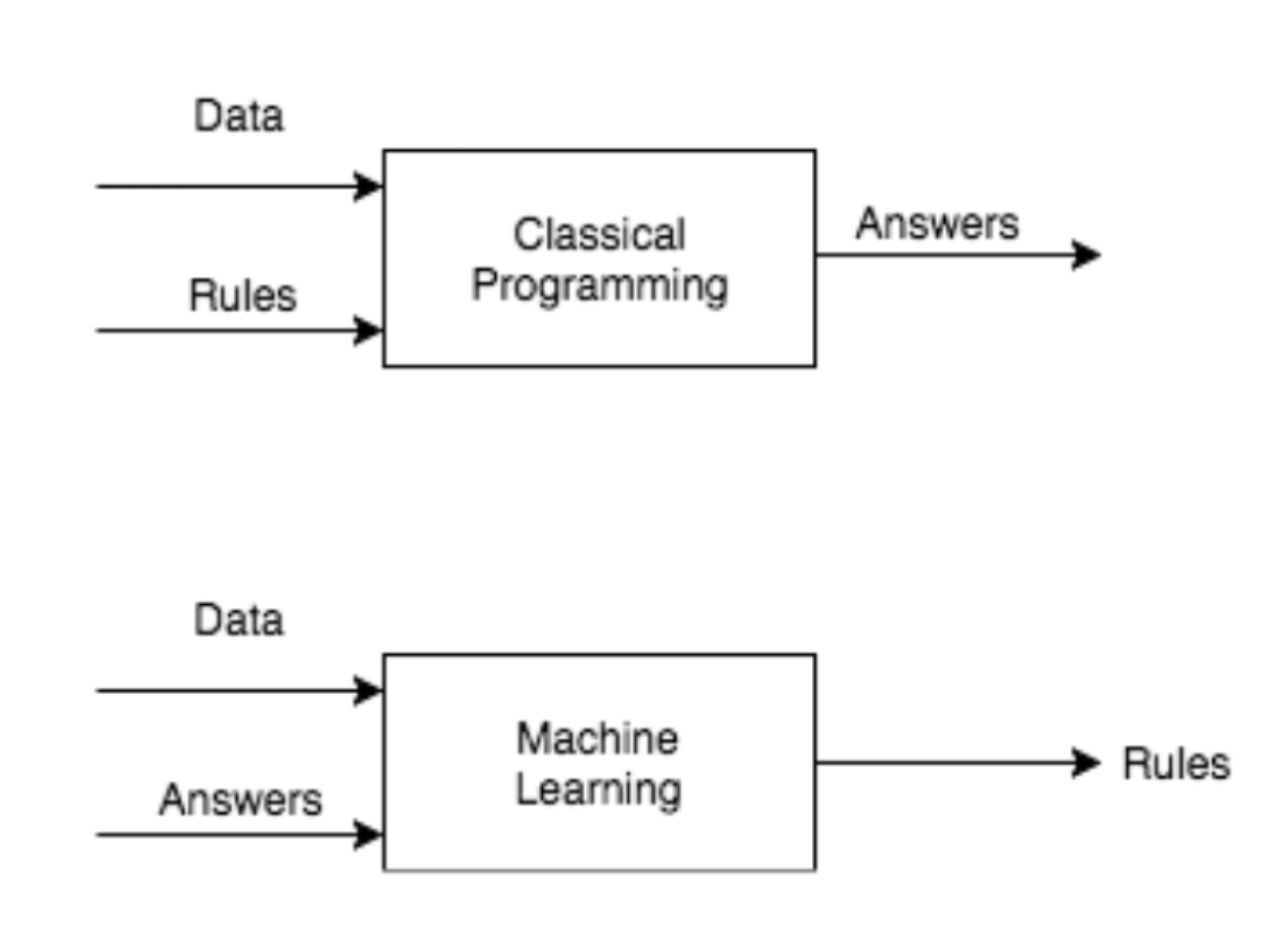
\includegraphics[width=0.8\textwidth]{./figures/ml-structure}
\caption{ML vs Traditional programming}
\label{fig:classicalvsmachinelearning}
\end{figure}

At a high level, machine learning systems took at tons of data and come up with rules to predict outcomes for unseen data as you can see in the figure ~\ref{fig:classicalvsmachinelearning}. 
Some examples of machine learning systems in the real life are:

\begin{itemize}
\item Google Photos uses a specific form of machine learning for grouping photos.
\item Recommendations systems which are family of ML algorithms. We can see this kind of recommendations systems in many famous apps like Spotify (music), Netflix (movies) and Amazon (products).
\end{itemize}

\subsection[Deep Learning]{Deep Learning}
Deep Learning is a sub-field of ML, that uses specific algorithms to extract features from images. They are based on neuronal networks whose inputs are each pixels of the image and they predict a label as an output.

For example, we can use the image of a number, the neuronal network will identify the borders of the number passing each pixel through the neuronal network's layers and it will determine which number is the image.

The use of DL has grown tremendously in the last few years with the rise of GPUs, big data, cloud providers (Amazon Web Services) and frameworks such as Torch, Tensorflow or Pytorch.

\newpage
\subsection[Reinforcement Learning]{Reinforcement Learning}

Reinforcement Learning is a sub-field of machine learning which addresses
the problem of automatic learning of optimal decisions over time. This is
a general and common problem studied in many scientific and engineering fields.\cite{reinforcement-learning}

Reinforcement Learning (RL) is the third camp and lays somewhere in between full supervision and a complete lack of predefined labels. On the one hand, it uses many well-established methods of supervised learning such as deep neural networks for function approximation, stochastic gradient descent, and back-propagation, to learn data representation.
On the other hand, it usually applies them in a different way. We need an agent that takes actions in some environment.

A good example of this is a robot mouse in a maze as you can see in the figure ~\ref{fig:maze}. Its environment is a maze with food at some points and electricity at others. 
The robot mouse can take actions such as turn left/right and move forward. Finally, at every moment it can observe the full state of the maze to make a 
decision about the actions it may take.
\begin{figure}[H]
\centering
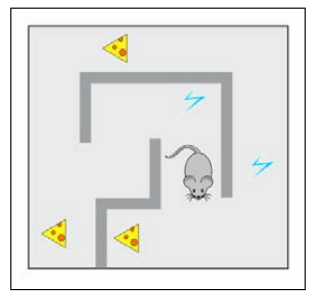
\includegraphics[width=0.5\textwidth]{./figures/robotmouse-maze}
\caption{Example of the Robot Mouse scenario \cite{reinforcement-learning}}
\label{fig:maze}
\end{figure}
It is trying to find as much food as  possible, while avoiding an electric shock whenever possible. These food and electricity signals stand as a reward given to the agent by the environment as additional feedback about the agent's actions.

\newpage
\section{State of the art}
\subsection[Neuronal network]{Neuronal network}

A neuronal network is a mathematical model that try to represents how our mind works. The first mathematical model was presented in 1943 called Perceptron this model could do several simple tasks \cite{fsancho}.

\begin{figure}[H]
\centering
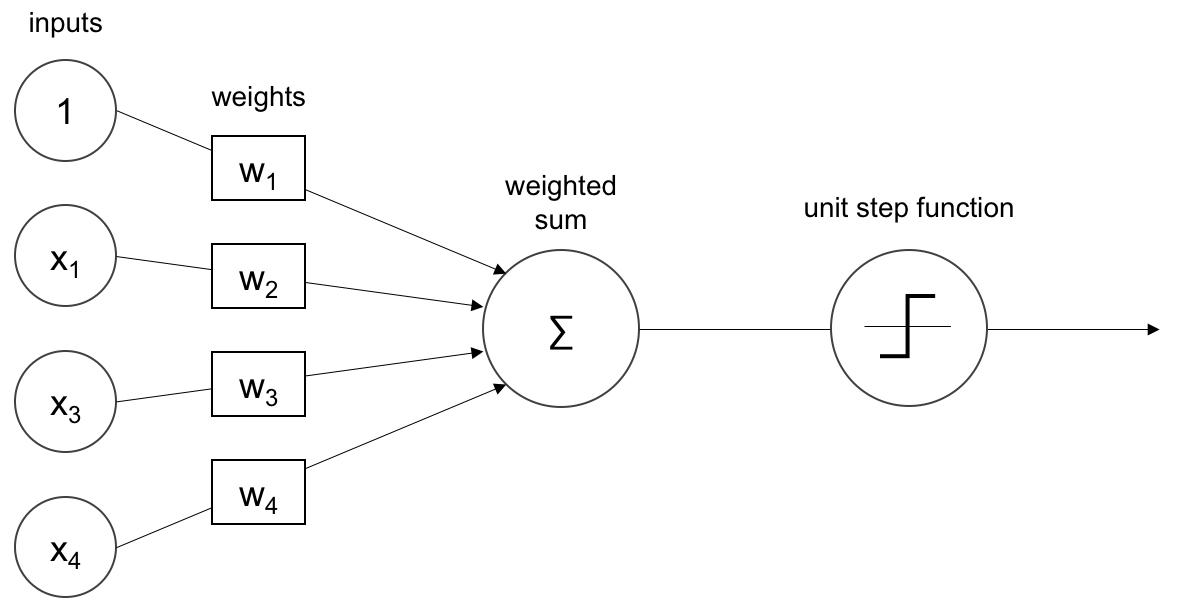
\includegraphics[width=0.8\textwidth]{./figures/perceptron}
\caption{Example of a perceptron \cite{rajalingappaa}}
\label{fig:perceptron}
\end{figure}
	
	
The figure ~\ref{fig:perceptron} represents a perceptron which has a set of inputs that are going to be multiplied by their weights.
Then the perceptron will perform a weighted summation to produce an output. \cite{sagar} Finally the output of the perceptron can be passed through an activation function or transfer function.\cite{rajalingappaa}
The process that the weight of the inputs changes in order to improve the output of the perceptron is called training. 

An Artificial Neuronal Network (ANN) is a collection of perceptrons as you can see in the figure ~\ref{fig:ann} and activation functions. The perceptrons are connected to form hidden layers or units. The hidden units form the non-linear basis that maps the input layers to output layers in a lower-dimensional space, which is also called artificial neural networks. ANN is a map from input to output. The map is computed by weighted addition of the inputs with biases. The values of weight and bias values along with the architecture are called model.

\begin{figure}[H]
\centering
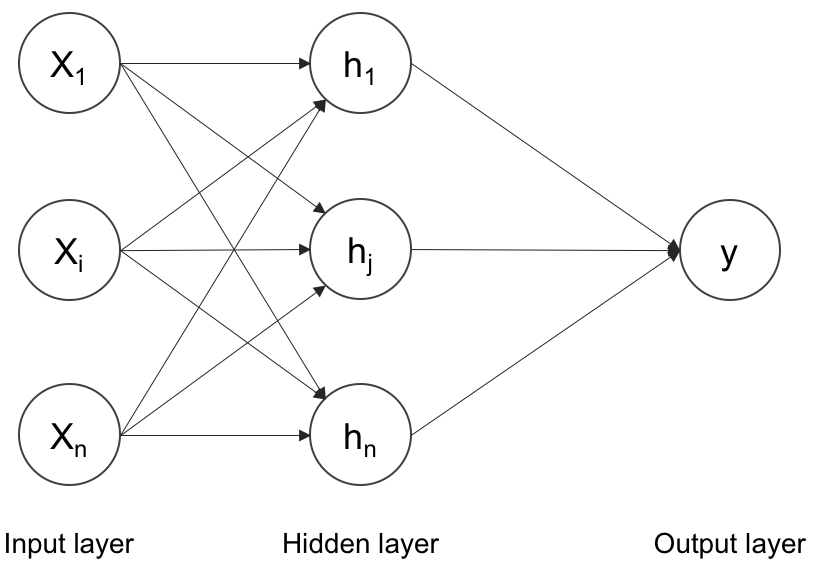
\includegraphics[width=0.8\textwidth]{./figures/ann}
\caption{Example of an Artificial Neuronal Network (ANN) \cite{rajalingappaa}}
\label{fig:ann}
\end{figure}
 
The ANN contains several parameters to optimize. The figure 
~\ref{fig:backpropragation} represents the procedure of updating the weights, this procedure is called back-propagation. The weights are updated from backward based on the error calculated. The procedure to minimize the error is called optimization.

\begin{figure}[H]
\centering
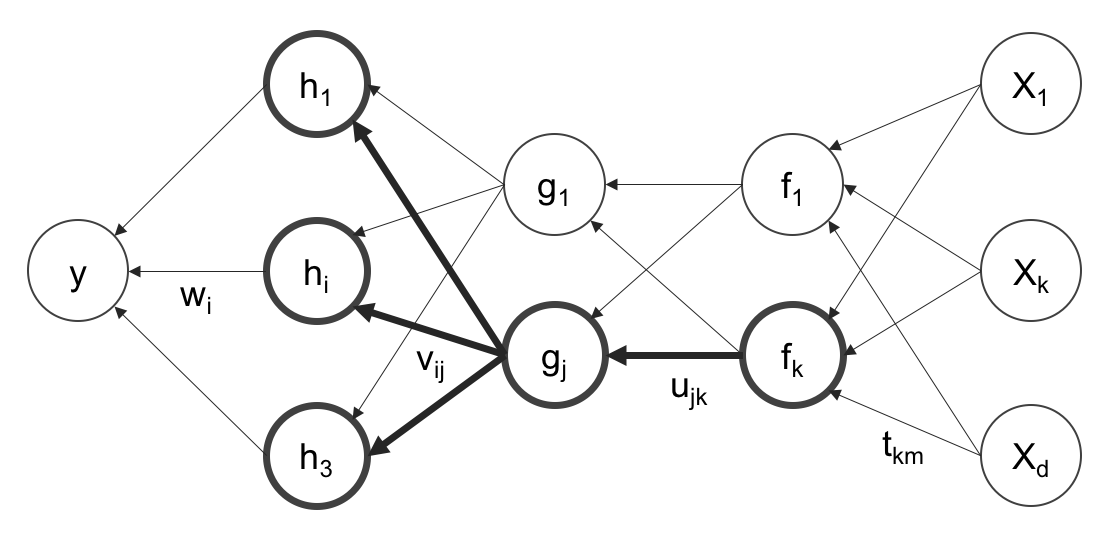
\includegraphics[width=0.8\textwidth]{./figures/backpropagation}
\caption{Example of back-propagation procedure \cite{rajalingappaa}}
\label{fig:backpropragation}
\end{figure}

   
A few different ANN models are available among them the Convolutional Neural Network (CNN) and Recurrent Neural Network (RNN). They have made some revolutionary improvements in the data analysis field. 

\subsection[Unsupervised Pretrained Networks]{Unsupervised Pretrained Networks}

\subsubsection[Autoencoders]{Autoencoders}

The figure ~\ref{fig:autoencoder} represents an autoencoder. It is an architecture for unsupervised learning. The main purpose of this architecture is to reduce the dimensionality of the dataset and it learns directly from the input data. 
The structure is very simple, the input layer followed by the bottleneck where the encoder and decoder operation are done and finally the output layer that contains the same number of units as the input layer does \cite{dp4j-deep-learning}.

\begin{figure}[H]
\centering
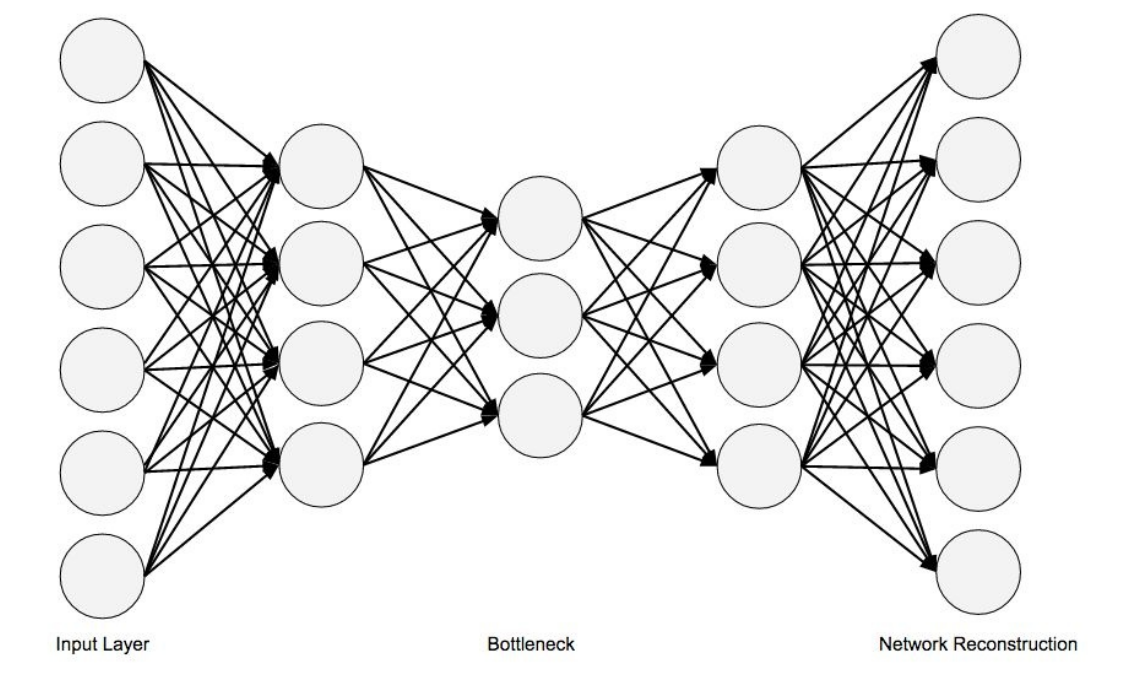
\includegraphics[width=0.8\textwidth]{./figures/autoencoder}
\caption{Example of Autoencoder \cite{dp4j-deep-learning}}
\label{fig:autoencoder}
\end{figure}


\subsubsection[Deep Belief Networks]{Deep Belief Networks}
Deep Belief Networks (DBNs) are composed of layer of Restricted Boltzmann Machines (RBMs).\\
A RBM is a neuronal network which can be useful for different kind of problems like dimensionality reduction, classification, regression, collaborative filtering, feature learning and topic modeling. The RBM is composed by two layers (visible layer and hidden layer). The nodes in the layer are not interconnected and each node starts making  stochastic decisions about whether to transmit that input or not, this is the main difference between the autoencoder and the RBM.

In unsupervised learning we use RBMs to extract high-level features from the input data. We discovered that if we let to RBMs to extract this high-level features it progressively can combine non-linear functions to extract more complex data, to understand better how it works we can see an example with MNIST digits \cite{dp4j-deep-learning}.

\subsection[Generative Adversarial Networks]{Generative Adversarial Networks}
The Generative Adversarial Networks is an example of unsupervised learning architecture where we train two models in parallel. Nowadays GANs architecture become really famous to create new images based on other images as you can see in the figure ~\ref{fig:monalisa} \cite{dp4j-deep-learning}. 

\begin{figure}[H]
\centering
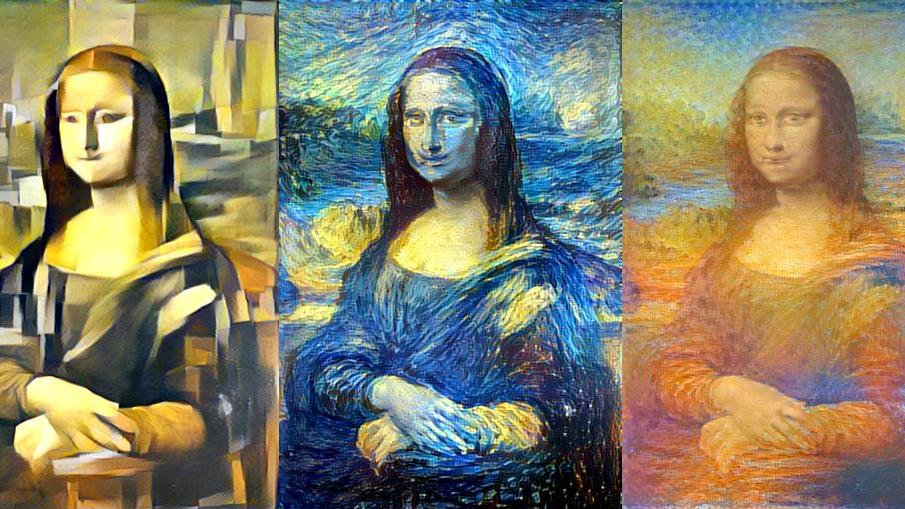
\includegraphics[width=0.8\textwidth]{./figures/monalisa}
\caption{Example of a GAN with The Mona Lisa painting \cite{can-art}}
\label{fig:monalisa}
\end{figure}

GAN is composed by two players, one player (the generator) generates samples that are similar to the training data without having access to that data and the second player (the discriminator) examine that samples and determine that data is real or fake \cite{can-art}.


\subsection[Convolutional Neuronal Network (CNN)]{Convolutional Neuronal Network (CNN)}


If we want to use a ANN for images the size of the network will be very large because of the number of neurons analysis will results an overfitting. Moreover in the case that we want to use big resolution images the size of the network will be huge \cite{rajalingappaa}.

The convolutional neuronal network (CNN) is an advance ANN, which allows the network to extract local as well as global features from the data, enhancing the decision-making procedure of the network\cite{abdullah}. As you can see in the figure ~\ref{fig:cnn} a CNN typically has convolutional layers interspersed with pooling (or sub-sampling) layers and then followed by fully connected layers as in a standard multi-layer neural network \cite{greenspan}.

\begin{figure}[H]
\centering
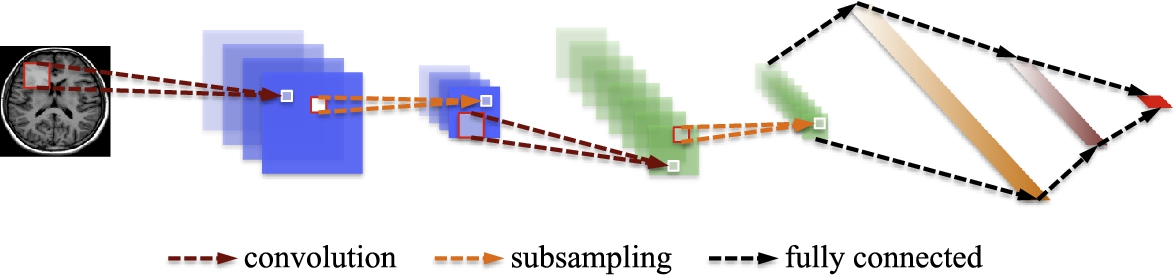
\includegraphics[width=0.8\textwidth]{./figures/cnn}
\caption{An architecture of a convolutional neural network}
\label{fig:cnn}
\end{figure}

\subsubsection[Convolution]{Convolution}

A convolution is defined as a mathematical operation describing a rule for how to merge two sets of information \cite{starteddeeplearning}.

\begin{figure}[H]
\centering
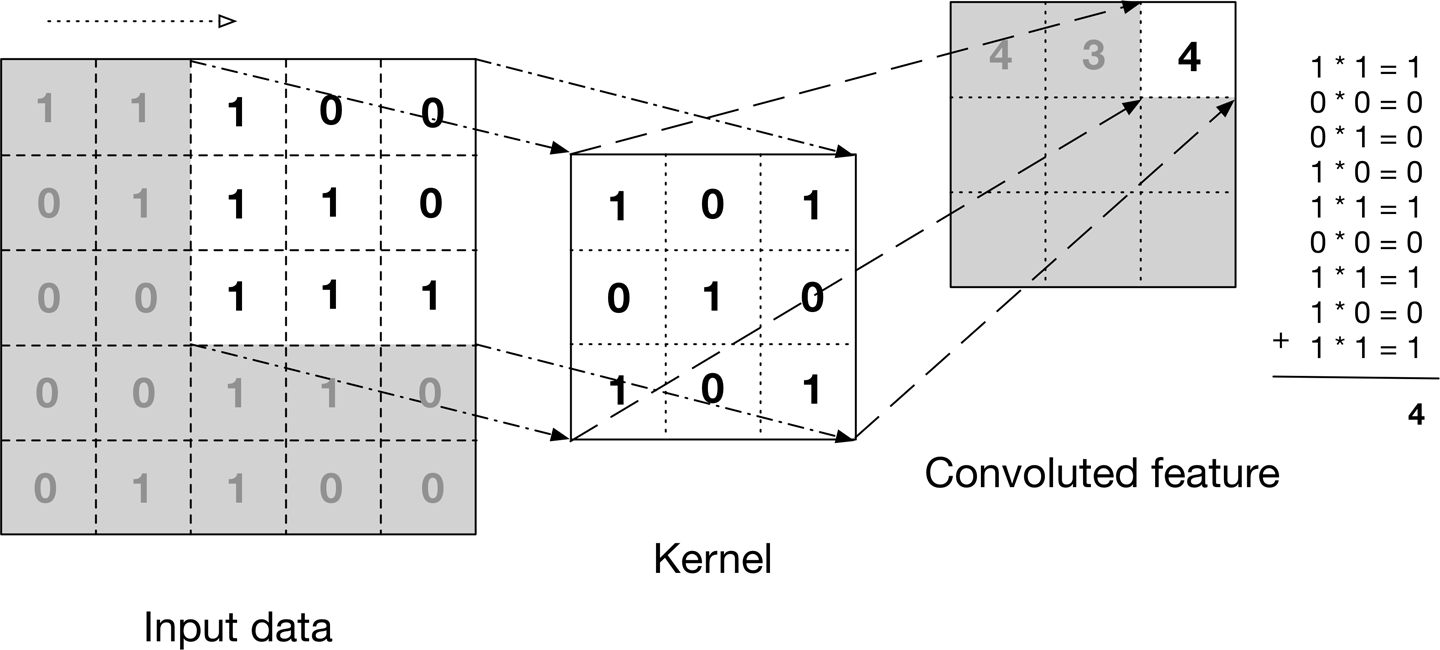
\includegraphics[width=0.8\textwidth]{./figures/convolution}
\caption{The convolution operation \cite{rajalingappaa}}
\label{fig:convolution}
\end{figure}

The figure \ref{fig:convolution} illustrate how the kernel is slid across the input data to produce the convoluted feature (output) data. 

\subsubsection[Pooling]{Pooling}

Usually after the convolution layer we will include a pooling layer to reduce the spatial size \cite{starteddeeplearning} (height and width) for the next layer. 
The most common pooling operation is max-pooling that reduces the size by a factor of $n^2$ \cite{greenspan} but exists other pooling operations like average-pooling, winner-takes-all pooling \cite{advancesneuralinformation} and stochastic pooling \cite{stochastic}. The figure ~\ref{fig:pooling} represents the max-pooling and the average-pooling operation for a better understanding.

\begin{figure}[H]
\centering
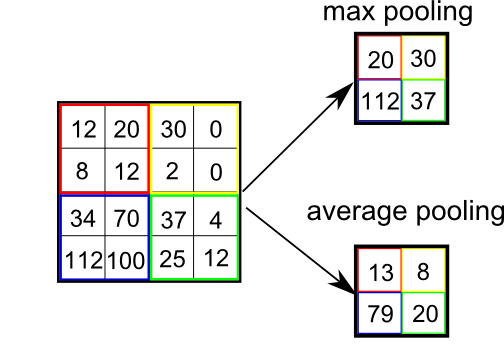
\includegraphics[width=0.8\textwidth]{./figures/pooling}
\caption{The max-pooling and average-pooling operation \cite{pooling}}
\label{fig:pooling}
\end{figure}

\subsubsection[Fully Connected Layers]{Fully Connected Layers}
We use this layer to compute class scores that we will use as output of the network. The dimension of the final output will be [1 x 1 x N] where N is the number of classes \cite{starteddeeplearning}. For example in our case the number of classes will be 2 (malignant or benign).




\section{Software}
There are many frameworks to resolve this problem. We are going to explain some for Python and compare them in order to choose the best framework to resolve our problem. 

\subsection[Tensorflow]{Tensorflow}
Tensorflow was created by the IA Google Team. They followed the same structure that Theano library, the engine was written in C/C++ to increase the speed \cite{generalcomparaison}
It support the CPU and GPU operations and you can run with multiple  GPU to optimize your model \cite{tensorflow}. Furthermore this library include a visualization of your model called Tensorboard so you are able to see how is training your model for debugging and optimization. Tensorflow is the most famous library for Machine Learning (ML) as you can see in the next figure ~\ref{fig:mentionsframeworks} works but, it's hard to learn and understand how it works in the beginning if we don't have any other experience in ML.


\begin{figure}[H]
\centering
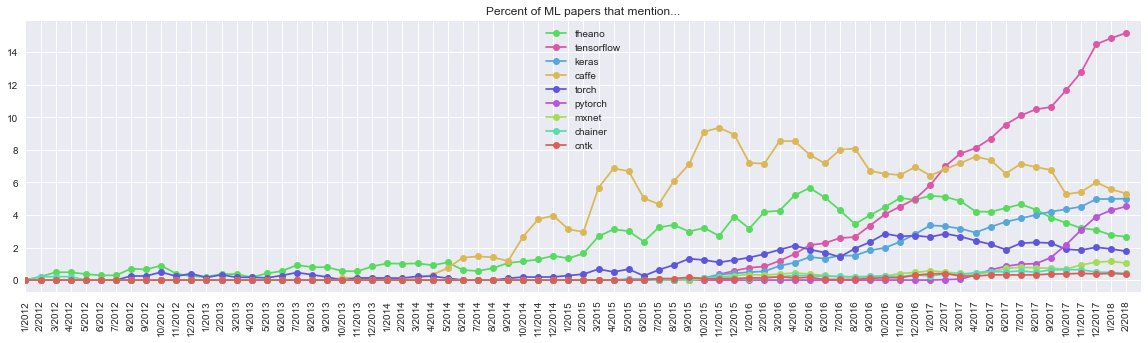
\includegraphics[width=1\textwidth]{./figures/libraries}
\caption{Percent of mentions in ML papers \cite{ml-mentions-image}}
\label{fig:mentionsframeworks}
\end{figure}


\subsection[Theano]{Theano}
Maintained by Montréal University group \cite{specificcomparaison} they were the pioneered to use a computational graph that will be use in Tensorflow project \cite{generalcomparaison}. In case for large models Theano will take long time to compute it, also it doesn't support multiple GPU. The error messages can be unhelpful so it will be hard for debugging tasks.

\subsection[Keras]{Keras}
Keras is an easy-to-use Python library \cite{specificcomparaison}
that sits atop Tensorflow and Theano so it took the advantages of both. It has an intuitive and simple API so you can write a model with a few lines of code. Keras is not really flexible and has some problems to use the multi-gpu. 

\subsection[Pytorch]{Pytorch}
The Python version of Torch called Pytorch is an open source project of Facebook created in January 2017. PyTorch has quickly become the favourite among machine learning researchers, because it allows certain complex architectures to be built easily  \cite{generalcomparaison}. Furthermore the modularity of Pytorch because it's easy to pull someone's code and use it \cite{specificcomparaison}. 

\subsection[H20]{H2O}
It's an open source software platform which core is coded in Java \cite{h20-deeplearning}
H20 is feature rich, ease of use and it's known for it's R and Spark integration but it provides support to other languages \cite{h20-comparative-table}.
H20 counts with other plugins to create an easy app after train your model (Shinny App).
 
\subsection[DL4J]{DL4J}
DL4J is a JVM-based, industry-focused, commercially supported, distributed deep learning framework \cite{generalcomparaison}. Python has many scientific environments to work with Deep Learning like Numpy or Theano but DL4J with Java and Scala has several advantages,
Java and Scala are inherently faster than Python. Anything written in Python by itself, disregarding its reliance on Cython, will be slower.
Furthermore the license under DL4J is Apache 2.0 License so anyone is free to make and patents derivative works based on Apache 2.0-licensed code. 

\section[Evaluate the model]{Evaluate the model}
There are many metrics and ways to evaluate the model and check the accuracy. Depends of the scenario we have to use a specific metric or other, there is not exist a metric for all the possibles scenarios. 
The objective of this section is to explain most of the famous metrics for a classification problem.

\subsection[Confusion Matrix]{Confusion Matrix}
This metric is the simplest because it's very easy to use and understand. Each column of the matrix represents the number of predictions for each class, while each row represents the instances in the actual class. One of the benefits of confusion matrices is that they make it easier to see if the system is confusing two classes.

The associated values of a confusion matrix are:

\begin{enumerate}
\item \textbf{True Positives (TP):} This happens when we give a positive diagnosis and the disease is present. In our case, the patient has melanoma lesion and we diagnose melanoma.
\item \textbf{True Negative (TN):}
This happens when we give a negative diagnosis and the disease is not present. In our case, the patient does not have melanoma and we diagnose not melanoma.
\item \textbf{False Positive (FP):} 
This happens when we give a positive diagnosis and the disease is not present. In our case, the patient does not have melanoma and we diagnose melanoma.
\item \textbf{False Negative (FP):} 
This happens when we give a negative diagnosis and the disease is present. In our case, the patient has melanoma and we diagnose not melanoma.
\end{enumerate}

Let's see an example of the confusion matrix to understand how it works. 
The scenario is a dog vs cat classification and the results are the following:
\begin{table}[H]
\centering
\begin{tabular}{llll}
\multicolumn{2}{l}{}                   & \multicolumn{2}{l}{Actual Class}  \\
\multicolumn{2}{l}{}                   & Cat & Dog                         \\
\multirow{2}{*}{Predicted Class} & Cat & 5   & 2                           \\
                                 & Dog & 3   & 3                          
\end{tabular}
\end{table}

\subsubsection[Sensitive]{Sensitive}
Measures the ability of a test to detect the condition when the condition is present.
\[ Sensitive = TP/(TP+FN) \]
In our cat classificator the sensitive is:
\[ Sensitive = 5/(5+3) = 0.625 \]

\begin{figure}[H]
\centering
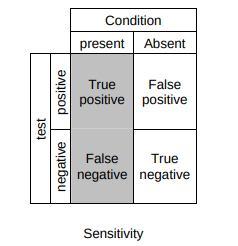
\includegraphics[width=0.3\textwidth]{./figures/Sensitive}
\caption{Calculate the Sensitive}
\end{figure}

\subsubsection[Specificity]{Specificity}
Measures the ability of a test to correctly exclude the condition (not detect the condition) when the condition is absent.
\[ Specificity  = TN/(TN+FP) \]
In our cat classificator the specificity is:
\[ Specificity = 3/(3+2) = 0.6 \]

\begin{figure}[H]
\centering
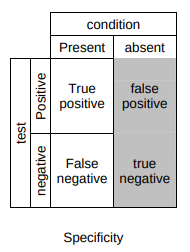
\includegraphics[width=0.3\textwidth]{./figures/Specificity}
\caption{Calculate the Specificity}
\end{figure}

\subsubsection[Predictive value positive]{Predictive value positive}
Measures the proportion of positives that correspond to the presence of the condition.
\[ PVP  =  TP/(TP+FP) \]
In our cat classificator the predictive value positive is:
\[ PVP = 5/(5+2) = 0.714 \]

\begin{figure}[H]
\centering
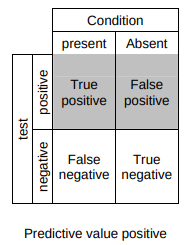
\includegraphics[width=0.3\textwidth]{./figures/PredictiveValuePositive}
\caption{Calculate the Predictive Value Positive}
\end{figure}


\subsubsection[Negative predictive value]{Negative predictive value}
Measures is the proportion of negatives that correspond to the absence of the condition. 
\[ NPV =  TN/(TN+FN) \]
In our cat classificator the predictive value negative is:
\[ NPV = 3/(3+3) = 0.5 \]

\begin{figure}[H]
\centering
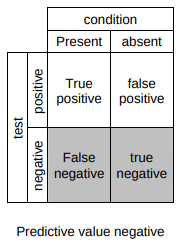
\includegraphics[width=0.3\textwidth]{./figures/PredictiveValueNegative}
\caption{Calculate the Predictive Value Negative}
\end{figure}

\subsection[The Area Under an ROC Curve]{The Area Under an ROC Curve}

The area under the ROC curve ( AUC ) is a measure of how well a parameter can distinguish between two diagnostic groups (diseased/normal). 

\begin{figure}[H]
\centering
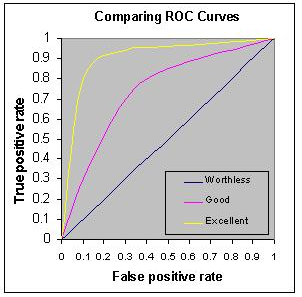
\includegraphics[width=0.3\textwidth]{./figures/ROC}
\caption{Examples of differents ROC curves \cite{area-roc-curve}}
\end{figure}

It's a famous metric in the health scenario, the accuracy is measured by the area under the ROC curve. An area of 1 represents a perfect test; an area of .5 represents a worthless test \cite{area-roc-curve}. A rough guide for classifying the accuracy of a diagnostic test is the traditional academic point system:

\begin{enumerate}
\item \textbf{.90 - 1} Excellent (A)
\item \textbf{.80 - .90} Good (B)
\item \textbf{.70 - .80} Fair (C)
\item \textbf{.60 - .70} Poor (D)
\item \textbf{.50 - .60} Fail (F)
\end{enumerate}


\section[Architectures]{Architectures}

Neural network can be compared with lego blocks, where you can build almost any simplex to complex structures. Actually, most of the famous architectures have been discovered during the 
\href{http://www.image-net.org/challenges/LSVRC/}{Large Scale Visual Recognition Challenge (ILSVRC)},  this challenge evaluates algorithms for object detection and image classification at large scale \cite{architectures}.

Depends of the task that we want to solve we have to use a type of architecture or other. The main types of tasks that computer vision can be categorised following the next figure \ref{fig:maintasks}.

\begin{figure}[H]
\centering
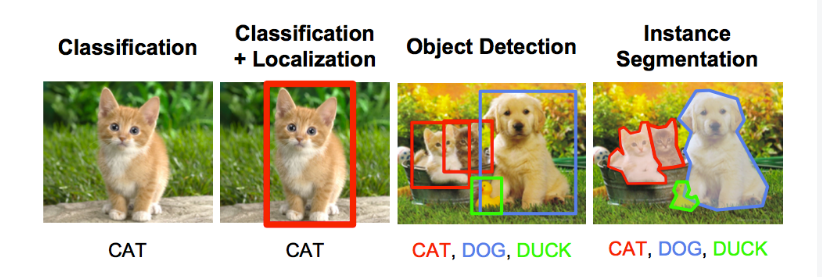
\includegraphics[width=0.7\textwidth]{./figures/Tasks-Architectures}
\caption{Examples of the main types of task in computer vision \cite{architectures}}
\label{fig:maintasks}
\end{figure}

\begin{enumerate}
\item \textbf{Object Recognition / Classification.} In object recognition, the goal is to identify the class givin a raw image.
\item \textbf{Classification + Localisation.} - In this one we have to identify the class and find the location of that object in the raw image.
\item \textbf{Object Detection.} The task is to identify where in the image does the objects lies in. 
\item \textbf{Image Segmentation.} It's a bit sophisticated task, where the objective is to map each pixel to its rightful class.
\end{enumerate}

\subsection[AlexNet]{AlexNet}

\begin{figure}[H]
\centering
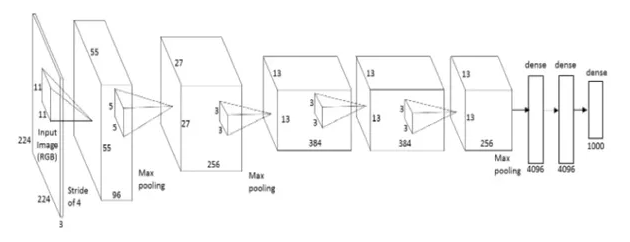
\includegraphics[width=0.6\textwidth]{./figures/Alexnet}
\caption{AlexNet Architecture \cite{advances-architectures}}
\label{fig:alexnet}
\end{figure}

It's the first deep architecture created by Geoffrey Hinton and his colleagues. When broken down, AlexNet seems like a simple architecture with convolutional and pooling layers one on top of the other, followed by fully connected layers at the top. This is a very simple architecture, as you can see in the figure ~\ref{fig:alexnet}, which was conceptualised way back in 1980s  \cite{advances-architectures}.

\subsection[VGG Net]{VGG Net}

\begin{figure}[H]
\centering
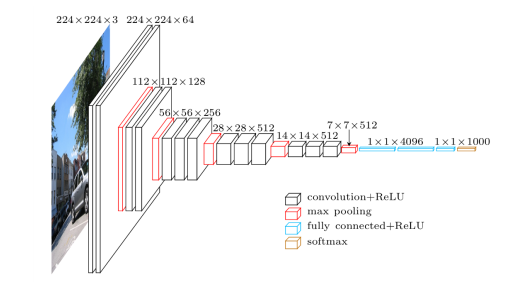
\includegraphics[width=0.6\textwidth]{./figures/VGGNet}
\caption{VGG Net Architecture \cite{advances-architectures}}
\label{fig:vgg}
\end{figure}
The figure ~\ref{fig:vgg} represents an architecture which was introduced by the researchers at Visual Graphics Group at Oxford (hence the name VGG).
The architecture is characterized by it's pyramidal shape, where the bottom layers which are closer to the image are wide, whereas the top layers are deep \cite{advances-architectures}.


\subsection[ResNet]{ResNet}

Residual Networks (ResNet in short) is an architecture composed by residual blocks that can preserve good results through the addition of layers. They solved a problem of accuracy saturation when you add many layers to the neuronal network, this problem is called vanish gradient.

\begin{figure}[H]
\centering
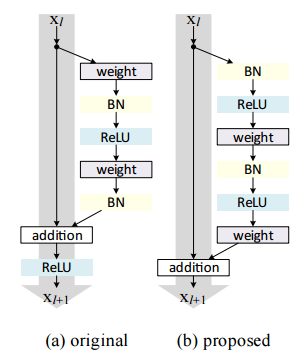
\includegraphics[width=0.4\textwidth]{./figures/ResNet}
\caption{ResNet Architecture \cite{advances-architectures}}
\label{fig:resnet}
\end{figure}

As you can see in the previous image ~\ref{fig:resnet} the main advantage of ResNet is that hundreds, even thousands of these residual layers can be used to create a network and then trained. This is a bit different from usual sequential networks, where you see that there is reduced performance upgrades as you increase the number of layers \cite{advances-architectures}.



%!TEX root =  tfg.tex
\chapter{Context}

\begin{abstract}
In this chapter we are going to explain the motivation, the main problem that we are going to solve. The development of the solution to the problem will be detailed, the results, plannification and costs for this solution.
\end{abstract}

\section[Motivation]{Motivation}

During my last year of degree I was wondering what I was going to work on my thesis. I knew I wanted to work on something related to health because I had always been interested in creating a product that would have an impact on society. 

In my internship I was in one of the most important research centres in France in the field of artificial intelligence. There I realized the potential of this technology that was emerging during these years and that I could do something related to health and that I had not worked previously during my studies.

The results expected at the end of this work will not have the same quality and precision work and studies recintes in the market (accuracy of 80\%-90\%) because we do not have the same resources as them. The main objective is to achieve a scalable prototype whose precision and quality will increase in the future.


\section[Problem]{Problem}
The problem that we are going to solve is a binary classification, we'll receive an image and we will detect if the image has skin cancer or not.
The objetives of this project is create a model based on deep learning algorithms to solve this problem, use different techniques to improve the accuracy and compare the obtained results with other algorithms or other works (papers, studies, etc). At the end we are going to expose the model in a REST API so we can use in the future for other projects, for example:

\begin{enumerate}
\item Create an app to take photos of skin moles and detect if there are skin cancer or not on it.
\item Monitor and collect more data for future studies (areas, age, gender affected by skin cancer...)
\end{enumerate}

\newpage
\section{ML Methodology}

This project is a machine learning project that is highly iteractive. It has some similarities as a software project. 

\begin{table*}[htb]
	\centering
	\begin{coolTable}{ll}{2}
{ML project structure}
	\textbf{Data collection and labeling}&Create labeling and validate quality of the data\\
	\textbf{Model exploration}&Start with a simple model and improve it\\
	\textbf{Testing and evaluation}&Revisit model evaluation metric\\
	\textbf{Model deployment}&Expose model as REST API, \\
	\textbf{Ongoing model maintenance}&Retrain model with new data to prevent model staleness\\
	\end{coolTable}
	\caption{Machine Learning project structure}
\end{table*}

\section[Data collection and labeling]{Data collection and labeling}

During this period we have to determine the feasibility of the project, in our case it's not a hard task to acquire the data, the ISIC institute exposed in 2018 more than 20.000 skin lesiono images during a challenge. 
\url{https://challenge2018.isic-archive.com/}
Furthermore exist other famous datasets like \emph{PH2Dataset} from the Oporto Universiy which the number of images is much lower but we can use some Data Augmentation techniques to improve the results.

\subsection[ISIC Dataset]{ISIC Dataset}

 

\part{Appendices}
\appendix


\lineNumbersOff

\glossarystyle{long}
\printglossaries
\newpage

\begin{thebibliography}{9}

\bibitem{ai-ml-dl-image} Pippa Biddle,Diamond Inc {\em https://bit.ly/2rkhRUY }, June 2017

  \bibitem{fsancho} Fernando Sancho Caparrini {\em http://www.cs.us.es/~fsancho/?e=72}  23 of April 2017.

  \bibitem{sagar} Sagar Sharma {\em https://towardsdatascience.com/what-the-hell-is-perceptron-626217814f53} 9 of September 2017.

  \bibitem{rajalingappaa} Rajalingappaa Shanmugamani {\em Deep learning for computer vision: expert techniques to train advanced neural networks using TensorFlow and Keras} 2018.

  \bibitem{abdullah} Abdullah-Al Nahid, Mohamad Ali Mehrabi, and Yinan Kong{\em Histopathological Breast Cancer Image Classification by Deep Neural Network Techniques Guided by Local Clustering} 7 March 2018.School of Engineering, Macquarie University, Sydney, Australia.

  \bibitem{greenspan} S. Kevin Zhou, Hayit Greenspan, Dinggang Shen
{\em Deep learning for medical image analysis} 2017.

  \bibitem{starteddeeplearning} Josh Patterson and Adam Gibson
{\em Getting started with deep learning } 2018.

\bibitem{reinforcement-learning} Maxim Lapan {\em Deep Reinforcement Learning Hands-On/}, June 2018

  \bibitem{advancesneuralinformation} R.K. Srivastava, J. Masci, S. Kazerounian, F. Gomez, J. Schmidhuber {\em Advances in Neural Information Processing Systems. } 2013.

  \bibitem{stochastic} M.D. Zeiler, R. Fergus{\em Stochastic pooling for regularization of deep convolutional neural networks. } 2013.

  \bibitem{ml-mentions-image} Andrej Karpathy {\em 
https://twitter.com/karpathy/status/972295865187512320?lang=es} March 2018

  \bibitem{generalcomparaison} {\em https://skymind.ai/wiki/comparison -frameworks-dl4j-tensorflow-pytorch}

  \bibitem{specificcomparaison} Vicky Kalogeiton Stéphane
Lathuilière, Pauline Luc Thomas, Lucas Konstantin Shmelkov
{\em https://project.inria.fr/deeplearning/files/2016/05/DLFrameworks.pdf} 25 of January 2017

 \bibitem{tensorflow} Tensorflow API
{\em https://www.tensorflow.org} 25 of January 2017

 \bibitem{stadisticframework} Andrej Karpathy 
{\em https://twitter.com/karpathy/status/972295865187512320}

\bibitem{area-roc-curve} The Area Under an ROC Curve definition 
{\em http://gim.unmc.edu/dxtests/roc3.htm}

\bibitem{architectures} Advanced Deep Learning Architectures Data
{\em https://www.analyticsvidhya.com/blog/2017/08/10-advanced-deep-learning-architectures-data-scientists/}

 
 \bibitem{h20-deeplearning} Srijan Agarwal
{\em https://opensourceforu.com/2017/01/introduction-h2o-relation-deep-learning/}, 21 of January 2018
 
 \bibitem{h20-comparative-table} Oksana Kutkina, Stefan Feuerriegel
{\em http://www.rblog.uni-freiburg.de/2017/02/07/deep-learning-in-r/}, 7 of March 2016 
 
 \bibitem{dp4j-deep-learning} Josh Patterson, Adam Gibson
{\em Deep Learning: A practitioner's approach/}, August 2017

\bibitem{can-art} Ahmed Elgammal, Bingchen Liu, Mohamed Elhoseiny, Marian Mazzone {\em CAN: Creative Adversarial Networks Generating “Art” by Learning About Styles and Deviating from Style Norms/}, August 2017

\end{thebibliography}



\end{document} 